
We show the first 2 layer weights in \figref{fig:quantization_for_actualweights}, and all results can be found in our \emph{supplementary}.
As shown in \figref{fig:quantization_for_actualweights}, On the classic five models, our ULQ has the lowest loss. From the actual model, most of the actual weights satisfy the normal distribution, especially the batch-norm-based models, whose weights are normally distributed, which means that the premise we made is reasonable.

\begin{figure*}[!ht]
    \flushleft
    \begin{minipage}[t]{1\textwidth}
            \flushleft
            \begin{overpic}[width=0.24\textwidth]{ActualWeights/Lenet-5/conv1/Distribution.pdf}
                \put(-10,15){\rotatebox{90}{Lenet-5}}
                \put(-10,-50){\rotatebox{90}{Cifarnet}}
                \put(-10,-115){\rotatebox{90}{Resnet-18}}
                \put(40,70){conv1}
                \put(145,70){loss}
                \put(250,70){conv2}
                \put(355,70){loss}
            \end{overpic}
            %\includegraphics[width=0.24\textwidth]{fig/SingleFmeasure/bark_f1_single.pdf}
            %\includegraphics[width=0.24\textwidth]{fig/Bitwidths/binary-results_1bit.pdf}
            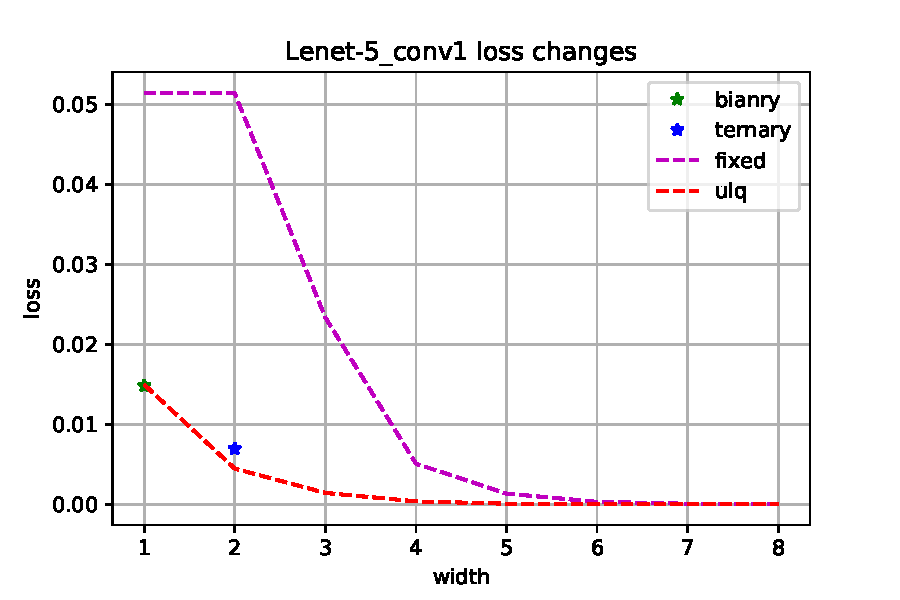
\includegraphics[width=0.24\textwidth]{ActualWeights/Lenet-5/conv1/LossWithWidth.pdf}
            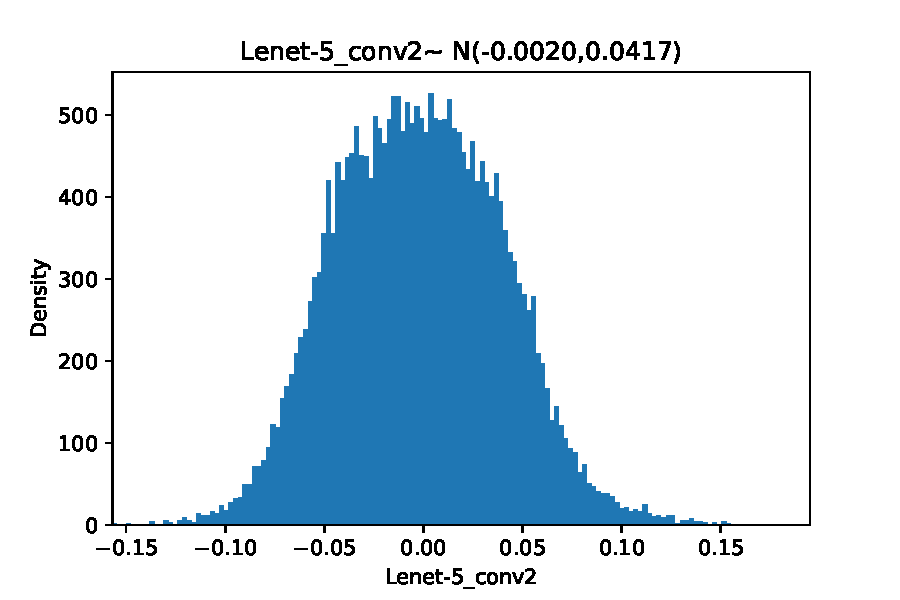
\includegraphics[width=0.24\textwidth]{ActualWeights/Lenet-5/conv2/Distribution.pdf}
            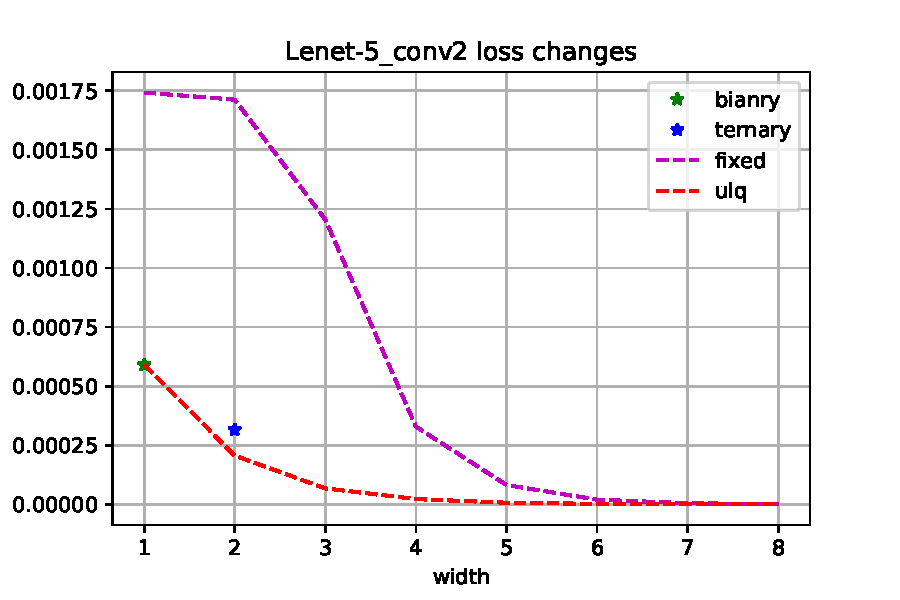
\includegraphics[width=0.24\textwidth]{ActualWeights/Lenet-5/conv2/LossWithWidth.pdf}\\
            
            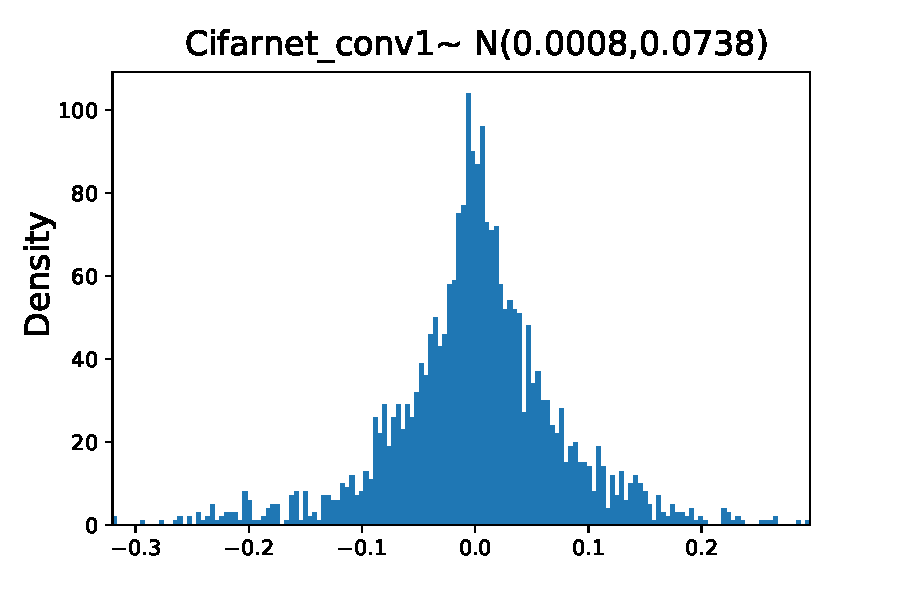
\includegraphics[width=0.24\textwidth]{ActualWeights/Cifarnet/conv1/Distribution.pdf}
            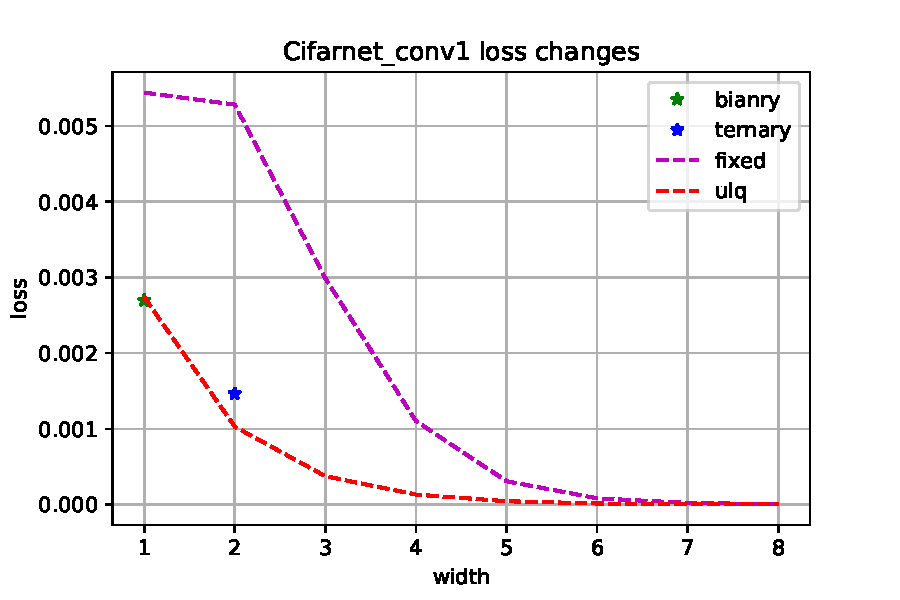
\includegraphics[width=0.24\textwidth]{ActualWeights/Cifarnet/conv1/LossWithWidth.pdf}
            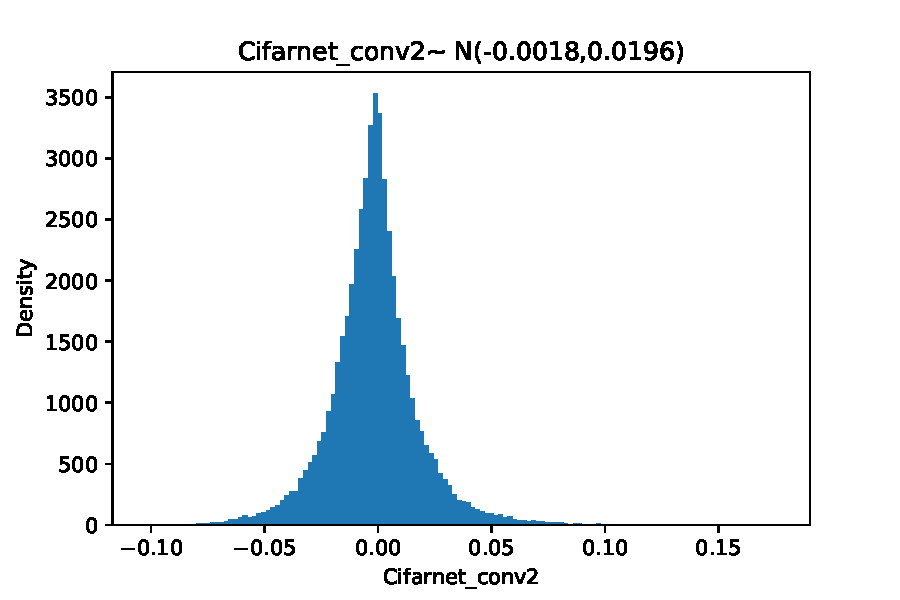
\includegraphics[width=0.24\textwidth]{ActualWeights/Cifarnet/conv2/Distribution.pdf}
            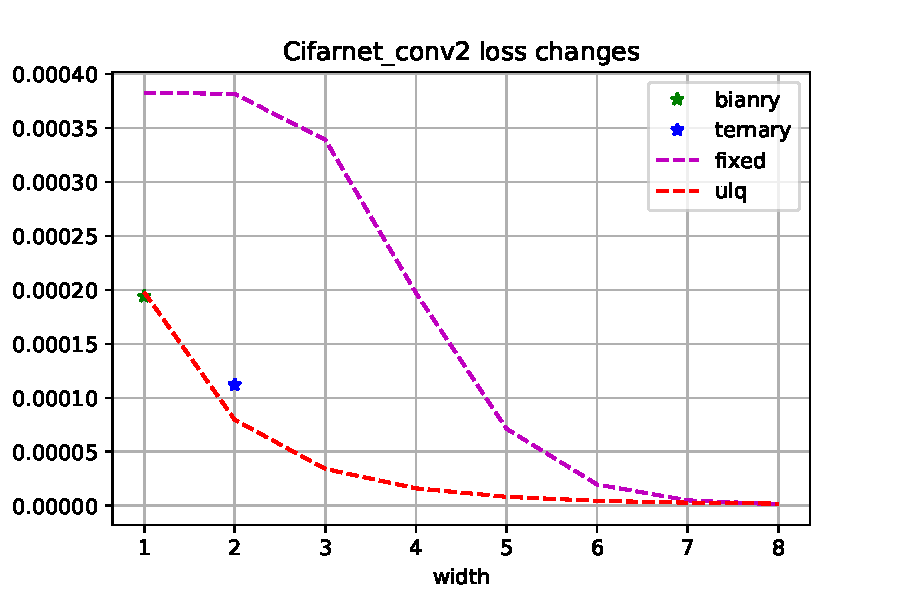
\includegraphics[width=0.24\textwidth]{ActualWeights/Cifarnet/conv2/LossWithWidth.pdf}\\
            
            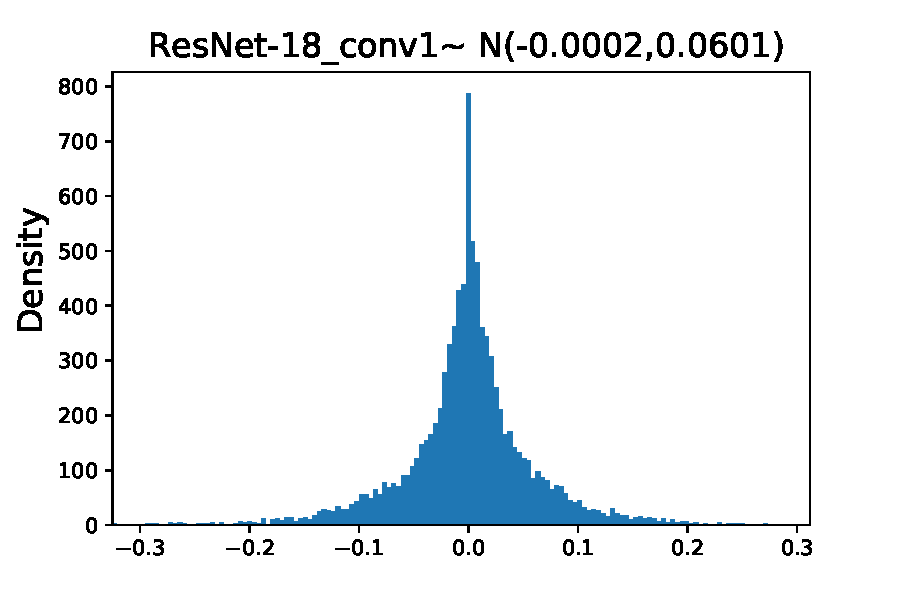
\includegraphics[width=0.24\textwidth]{ActualWeights/Resnet-18/conv1/Distribution.pdf}
            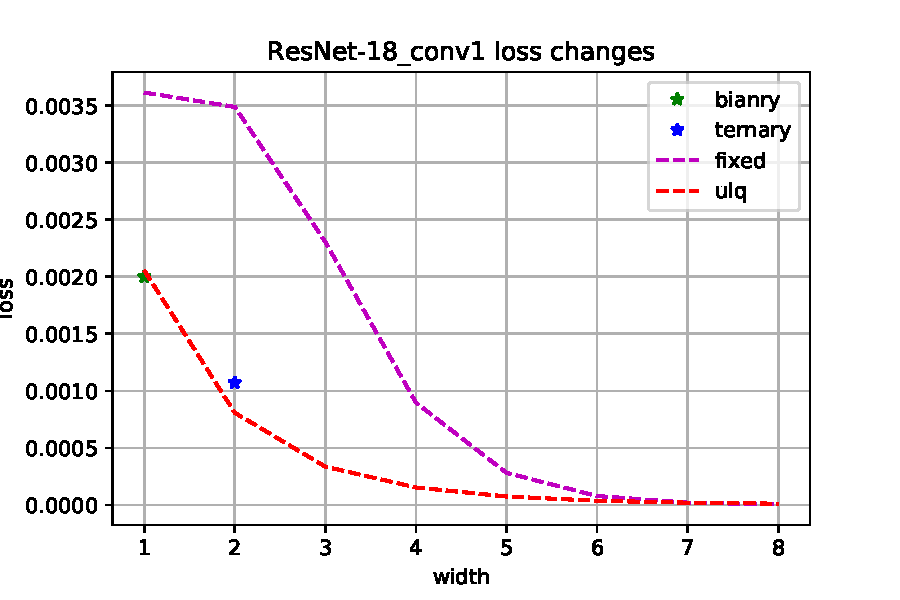
\includegraphics[width=0.24\textwidth]{ActualWeights/Resnet-18/conv1/LossWithWidth.pdf}
            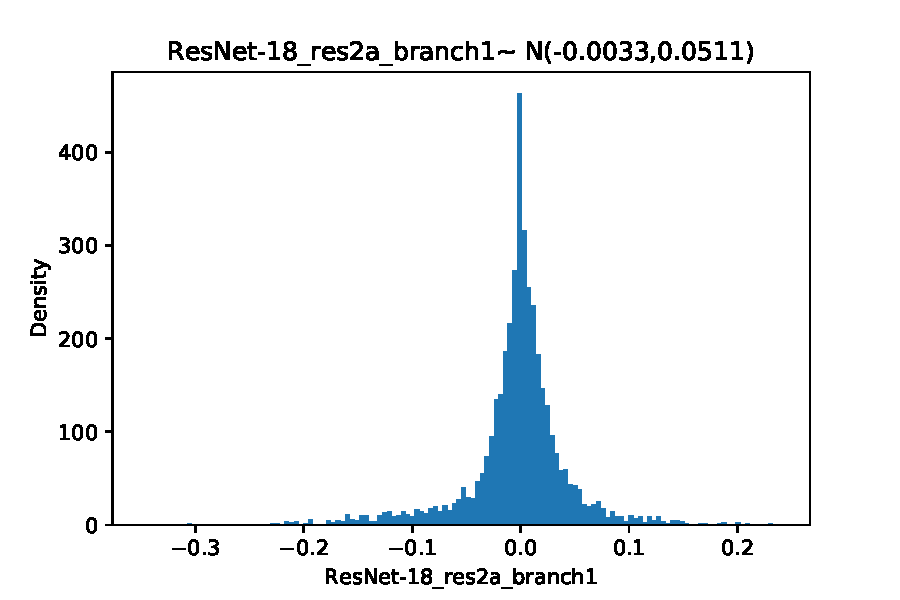
\includegraphics[width=0.24\textwidth]{ActualWeights/Resnet-18/branch1/Distribution.pdf}
            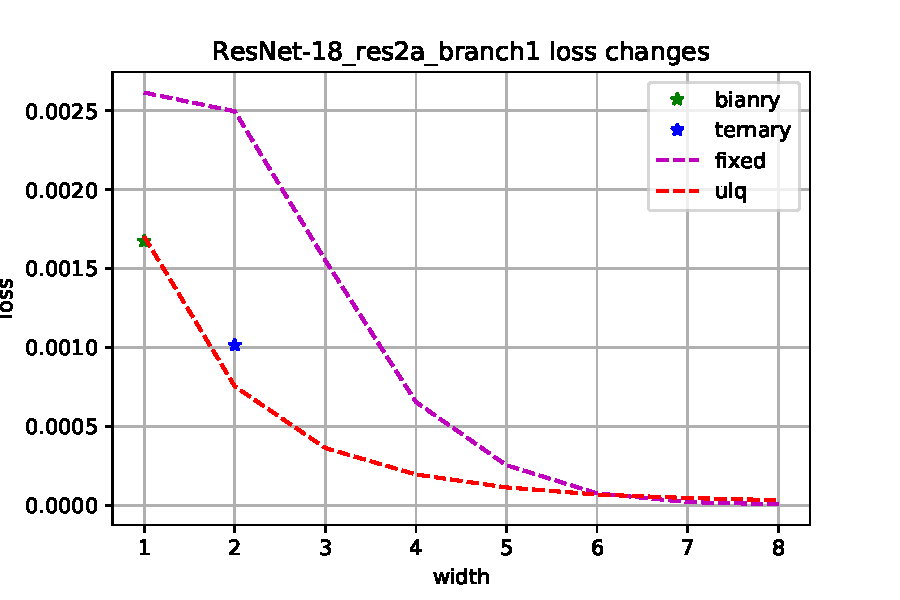
\includegraphics[width=0.24\textwidth]{ActualWeights/Resnet-18/branch1/LossWithWidth.pdf}
            %\fbox{\rule[-. 5cm]{0cm}{4cm} \rule[-. 5cm]{4cm}{0cm}}
    \end{minipage}
    \caption{Quantization comparision for the first 2 layers of models. All the weights satisfy the normal distribution and ULQ keeps the lowest loss in all results.}
    \label{fig:quantization_for_actualweights}
\end{figure*}